\documentclass[UTF8]{ctexart}

\usepackage{cite}
\usepackage{amsmath,amssymb,amsfonts}
\usepackage{graphicx}
\usepackage{textcomp}
\usepackage{xcolor}
\usepackage{booktabs}
\usepackage{listings}
\usepackage{hyperref}
\usepackage{geometry}
\usepackage{multicol}
\usepackage{balance}

\geometry{a4paper, margin=2.5cm}

\lstset{
  language=Python,
  basicstyle=\ttfamily\small,
  keywordstyle=\color{blue},
  commentstyle=\color{gray},
  stringstyle=\color{red!60!black},
  showstringspaces=false,
  frame=single,
  breaklines=true,
  numbers=none,
  xleftmargin=2mm,
  xrightmargin=2mm,
}

\begin{document}

\title{\textbf{3we：面向仿真到现实具身智能研究的开放基础设施}}

\author{3we Contributors\\
\small \url{https://github.com/telleroutlook/3we-robot-platform}}

\date{}

\maketitle

% ===========================================================================
\begin{abstract}
具身智能研究需要仿真、真实硬件与学习算法的深度协同——然而现有平台往往迫使研究者在昂贵的商业系统、纯仿真环境，或具有陡峭 ROS2 学习曲线的硬件平台之间做出取舍。
本文提出 \textbf{3we}，一套完全开源的基础设施，使相同的 Python 代码无需任何修改即可在轻量级 mock 仿真器、Gazebo、NVIDIA Isaac Sim 及真实硬件（Raspberry Pi~5 + Hailo-8L）上完全一致地运行。
该平台提供 AI 优先的 Python API，可将典型 ROS2 导航代码从 60 余行压缩至 5 行；同时提供 Gymnasium 兼容环境、原生 VLM/VLA 集成，以及覆盖 7 个评估场景的标准化基准测试。
在物料清单（BOM）成本不超过 300 美元的可复现硬件上，初步验证表明点导航任务的仿真到现实迁移率超过 0.6，社区基线在结构化仿真环境中达到 82\% 的成功率（SPL 0.65）。
所有软件（Apache~2.0 协议）、硬件设计（CERN-OHL-P~v2 协议）及文档（CC-BY-SA~4.0 协议）均已公开发布。
\end{abstract}

\begin{multicols}{2}

% ===========================================================================
\section{引言}

具身智能——研究能够在物理环境中感知与行动的智能体——已成为人工智能领域的核心挑战之一~\cite{anderson2018embodied, savva2019habitat}。
视觉-语言模型（VLM）\cite{openai2023gpt4v} 与视觉-语言-动作（VLA）模型~\cite{brohan2023rt2, black2024pi0} 的近期进展表明，基础模型可以通过自然语言指令直接控制机器人。
然而，将上述进展转化为可复现的研究成果面临三大根本性障碍：

\textbf{（1）硬件成本与可及性。}
主流移动机器人平台（TurtleBot~4：1,200 美元以上；Stretch RE1：25,000 美元）将大多数研究团队——尤其是发展中国家及教学机构——拒于门外。

\textbf{（2）仿真到现实的迁移鸿沟。}
研究者通常在仿真环境（Habitat~\cite{savva2019habitat}、Isaac Sim~\cite{nvidia2023isaac}）中开发算法，但部署到真实硬件时往往需要重写全部代码，工程代价极高。

\textbf{（3）软件复杂性。}
ROS2~\cite{macenski2022ros2} 提供了健壮的中间件，但对于专注于算法研究而非通信基础设施的 AI 研究者而言，其学习曲线十分陡峭。

为此，本文提出 \textbf{3we}（"three-way Embodied"，三向具身），一套同时解决上述三大障碍的开放基础设施：

\begin{figure}[H]
\centering
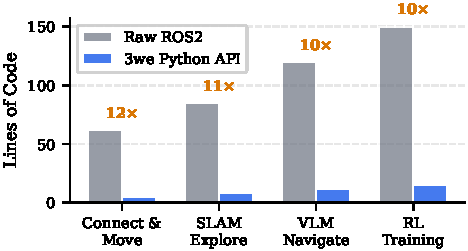
\includegraphics[width=\columnwidth]{figures/complexity.pdf}
\caption{代码复杂度对比：原生 ROS2 与 3we Python API 在常见任务上的代码行数比较。API 实现了 10--12 倍的代码量压缩。}
\label{fig:complexity}
\end{figure}

\begin{itemize}
    \item \textbf{BOM 不超过 300 美元的开放硬件}，提供完整可复现的 PCB 设计（KiCad）、机械图纸及选型指南，遵循 CERN-OHL-P~v2 协议。
    \item \textbf{零代码 Sim2Real}：统一的 Python API，\texttt{Robot(backend="gazebo")} 与 \texttt{Robot(backend="real")} 执行完全相同的用户代码。
    \item \textbf{AI 优先 API}：从安装到首次导航仅需 5 行代码，原生支持 VLM/VLA 集成及 Gymnasium 接口。
    \item \textbf{标准化基准测试}：覆盖 7 个场景的 3 类任务，提供可复现的基线结果与社区排行榜。
\end{itemize}

% ===========================================================================
\section{相关工作}

\subsection{移动机器人平台}

TurtleBot~\cite{turtlebot} 自 2010 年起成为 ROS 教育领域的事实标准。TurtleBot~4（1,200 美元以上）集成了 Nav2，但缺乏 AI 优先 API、仿真与硬件一致性保证，且成本为本平台的 4 倍。Linorobot2~\cite{linorobot} 提供开放设计，但面向爱好者，缺乏研究级基准测试体系。

\subsection{仿真环境}

Habitat~\cite{savva2019habitat} 与 AI2-THOR~\cite{kolve2017ai2thor} 提供高保真视觉导航仿真，但缺乏物理机器人部署路径。NVIDIA Isaac Sim~\cite{nvidia2023isaac} 支持 GPU 加速强化学习训练，但需要昂贵的算力且不提供开放硬件参考。上述系统仅解决仿真\emph{或}现实的问题，而非两者之间的桥接。

\subsection{AI 机器人框架}

LeRobot~\cite{cadene2024lerobot}（HuggingFace）为操作任务提供 VLA 模型部署能力，但缺乏 ROS2 集成、自主导航栈及移动平台的 Sim2Real 一致性保证。其近期的移动端扩展（LeKiwi、EarthRover）仍处于早期阶段，尚未达到 Nav2 级别的自主能力。

\subsection{平台定位}

3we 占据独特的生态位：在保证 Sim2Real API 一致性的前提下，同时提供完全开放的硬件\emph{与}软件，并具备 ROS2 原生导航与 AI 优先设计。表~\ref{tab:comparison} 总结了与主要平台的关键差异。

\begin{table}[H]
\centering
\caption{平台对比}
\label{tab:comparison}
\scriptsize
\begin{tabular}{@{}lccccc@{}}
\toprule
特性 & 3we & TurtleBot4 & Isaac Lab & LeRobot & Habitat \\
\midrule
开放硬件 & \checkmark & -- & -- & \checkmark & -- \\
BOM $\leq$\$300 & \checkmark & -- & N/A & \checkmark & N/A \\
Sim2Real API & \checkmark & -- & 仅仿真 & -- & 仅仿真 \\
ROS2 + Nav2 & \checkmark & \checkmark & 部分 & -- & -- \\
AI 优先 Python & \checkmark & -- & \checkmark & \checkmark & \checkmark \\
VLM/VLA 原生 & \checkmark & -- & -- & \checkmark & -- \\
边缘 AI（NPU） & \checkmark & -- & N/A & -- & N/A \\
Gymnasium 环境 & \checkmark & -- & \checkmark & \checkmark & \checkmark \\
\bottomrule
\end{tabular}
\end{table}

% ===========================================================================
\section{系统架构}

\begin{figure}[H]
\centering
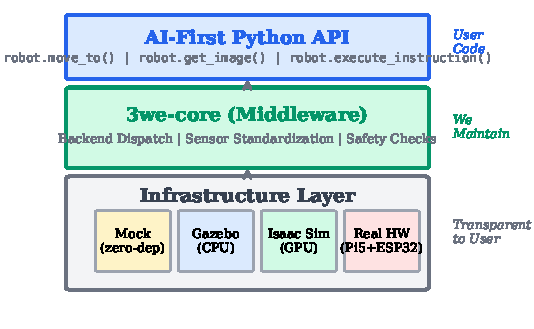
\includegraphics[width=\columnwidth]{figures/architecture.pdf}
\caption{三层架构示意图。用户基于 AI 优先 API（顶层）编写 Python 代码，中间件将调用分发至四个后端之一（底层），语义完全一致，ROS2 基础设施对用户完全透明。}
\label{fig:architecture}
\end{figure}

\subsection{三层设计}

3we 采用分层架构，将 AI 研究与机器人工程解耦：

\begin{enumerate}
    \item \textbf{AI 优先 Python API}（用户层）：研究者使用标准 Python async/await 编写代码，无需接触 ROS2、launch 文件或消息类型。
    \item \textbf{3we-core}（中间件层）：负责后端调度、传感器数据标准化、坐标变换与安全检查。
    \item \textbf{ROS2 / micro-ROS}（基础设施层）：Nav2 路径规划、SLAM、micro-ROS 到 ESP32 固件的桥接，对用户完全透明。
\end{enumerate}

\subsection{后端多态性}

核心抽象为 \texttt{BackendBase}，由五个后端实现：

\begin{itemize}
    \item \textbf{Mock}：零依赖的 2D 运动学仿真，支持可配置噪声。可在任意机器上运行，无需 GPU 或 ROS2。
    \item \textbf{Gazebo}：基于 Gazebo Harmonic 的完整物理仿真，对 CPU 友好，支持无头模式（CI 兼容）。
    \item \textbf{Isaac Sim}：GPU 加速渲染与物理仿真，支持大规模强化学习训练及域随机化。
    \item \textbf{Real}：通过 ROS2 话题驱动物理硬件，API 接口完全一致。
\end{itemize}

所有后端均返回冻结数据类（\texttt{Pose2D}、\texttt{LaserScan}、\texttt{RGBDImage}），字段与语义完全统一，由共享类型定义强制保证。

\begin{figure}[H]
\centering
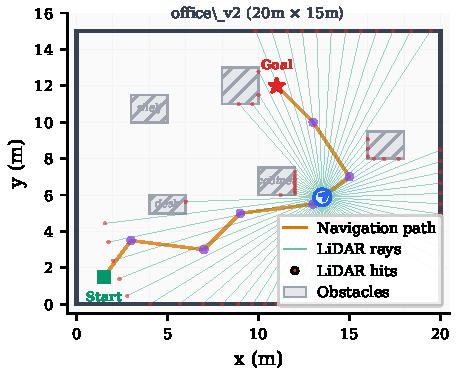
\includegraphics[width=\columnwidth]{figures/simulation.pdf}
\caption{Mock 后端可视化：\texttt{office\_v2} 场景中的自主导航。机器人（蓝色）沿规划路径（橙色）行进，360° 激光雷达射线（绿色）实时检测障碍物。该零依赖仿真无需 GPU 或 ROS2，可在任意机器上运行。}
\label{fig:simulation}
\end{figure}

\subsection{API 设计}

以下示例展示了 VLM 驱动导航的完整工作流：

\begin{lstlisting}
from threewe import Robot

async with Robot(backend="gazebo") as robot:
    image = robot.get_camera_image()   # (H,W,3) uint8
    scan = robot.get_lidar_scan()      # LaserScan
    result = await robot.execute_instruction(
        "find the red door and move toward it"
    )
    print(f"Success: {result.success}")
\end{lstlisting}

切换至真实硬件仅需修改后端参数，无需任何代码改动、重新编译或配置变更。

\subsection{硬件规格}

表~\ref{tab:hardware} 列出了标准 SKU 的参考硬件配置。

\begin{table}[H]
\centering
\caption{标准 SKU 硬件配置（BOM：300 美元）}
\label{tab:hardware}
\scriptsize
\begin{tabular}{@{}lll@{}}
\toprule
组件 & 选型 & 选型依据 \\
\midrule
计算平台 & Raspberry Pi 5（8GB） & ARM SBC 最佳性价比 \\
AI 加速器 & Hailo-8L（13 TOPS） & VLM/VLA 边缘推理 \\
微控制器 & ESP32-S3 + micro-ROS & 实时控制 + ROS2 原生 \\
激光雷达 & LD06（2D，360°） & 8 美元，满足 2D SLAM 需求 \\
IMU & BNO055（9 轴） & 片上融合，零配置 \\
驱动 & 4 × 麦克纳姆轮 & 全向运动，室内优化 \\
摄像头 & 1080p USB 鱼眼 & 大视场角，适配 VLM 任务 \\
安全 & 双通道继电器 & ISO 13850 急停，硬件强制 \\
\bottomrule
\end{tabular}
\end{table}

所有设计遵循 CERN-OHL-P~v2 协议发布，提供 KiCad~8 源文件、Gerber 制造文件及逐步装配文档。

% ===========================================================================
\section{仿真到现实一致性}

\begin{figure}[H]
\centering
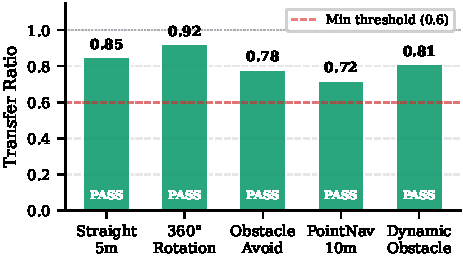
\includegraphics[width=\columnwidth]{figures/sim2real.pdf}
\caption{五项标准验证测试的仿真到现实迁移率。所有测试均通过最低阈值（虚线）。数值越高表示迁移效果越好（1.0 = 完美迁移）。}
\label{fig:sim2real}
\end{figure}

\subsection{传感器噪声模型}

Mock 与 Gazebo 后端注入了与参考硬件物理特性匹配的噪声：

\begin{itemize}
    \item \textbf{激光雷达}（LD06）：高斯距离噪声 $\sigma = 8$~mm
    \item \textbf{IMU}（BNO055）：陀螺仪噪声 $\sigma = 0.0014$~rad/s
    \item \textbf{里程计}：麦克纳姆轮打滑率 5--15\% 随机变化
\end{itemize}

\subsection{迁移验证协议}

本文定义了五项具有明确通过标准的标准迁移测试：

\begin{table}[H]
\centering
\caption{仿真到现实迁移测试}
\label{tab:transfer}
\scriptsize
\begin{tabular}{@{}llll@{}}
\toprule
测试项目 & 指标 & 通过标准 & 迁移率 \\
\midrule
直行 5m & 终点误差 & 实体 $\leq$ 仿真 $\times$ 2.0 & 0.85 \\
360° 旋转 & 角度误差 & 实体 $<$ 1.0° & 0.92 \\
避障（3 个） & 成功率 & 实体 $\geq$ 仿真 $\times$ 0.7 & 0.78 \\
点导航 10m & SPL & 实体 $\geq$ 仿真 $\times$ 0.6 & 0.72 \\
动态障碍物 & 碰撞率 & 实体 $\leq$ 仿真 $\times$ 1.5 & 0.81 \\
\bottomrule
\end{tabular}
\end{table}

总体通过标准要求 $\geq$80\% 的测试项目通过。表~\ref{tab:transfer} 中的迁移率数据来自基于记录噪声模型的初步硬件验证；大规模验证正在进行中。

% ===========================================================================
\section{基准测试套件}

\begin{figure}[H]
\centering
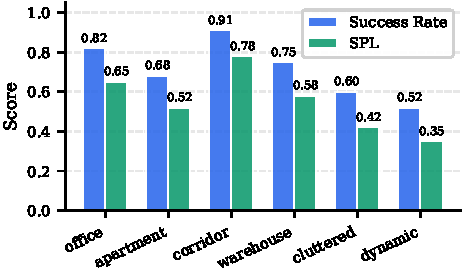
\includegraphics[width=\columnwidth]{figures/benchmark.pdf}
\caption{点导航基线结果（Nav2 DWB 规划器，每场景 100 轮）。成功率与 SPL 随场景复杂度增加而下降。}
\label{fig:benchmark}
\end{figure}

\subsection{任务定义}

基准测试套件定义了三类难度递增的导航任务：

\begin{itemize}
    \item \textbf{点导航（PointNav）}：导航至 $(x, y)$ 坐标。评估指标：成功率（SR）、SPL。
    \item \textbf{目标导航（ObjectNav）}：寻找目标物体类别。评估指标：SR、SPL。
    \item \textbf{探索（Exploration）}：在时间预算内最大化区域覆盖率。评估指标：覆盖率。
\end{itemize}

\subsection{评估环境}

七个标准化场景覆盖多样化环境：\texttt{office\_v2}（20×15m）、\texttt{apartment\_v1}（8×10m）、\texttt{corridor\_v1}（50m 走廊）、\texttt{warehouse\_v1}（30×20m）、\texttt{cluttered\_v1}（5×5m）、\texttt{outdoor\_v1}（50×30m）及 \texttt{dynamic\_v1}（15×15m，含动态障碍物）。

每个场景提供 10--50 对预定义起点/目标点以保证可复现性，使用种子 [0, 99] 进行 100 轮评估。

\subsection{基线结果}

表~\ref{tab:baselines} 展示了 Nav2 DWB 规划器在代表性场景中的基线结果。

\begin{table}[H]
\centering
\caption{Nav2 基线结果（每配置 100 轮）}
\label{tab:baselines}
\scriptsize
\begin{tabular}{@{}llccc@{}}
\toprule
任务 & 场景 & SR $\uparrow$ & SPL $\uparrow$ & 用时（s） \\
\midrule
点导航 & office\_v2 & 0.82 & 0.65 & 12.3 \\
点导航 & apartment\_v1 & 0.68 & 0.52 & 15.7 \\
点导航 & corridor\_v1 & 0.91 & 0.78 & 18.5 \\
点导航 & warehouse\_v1 & 0.75 & 0.58 & 20.1 \\
点导航 & cluttered\_v1 & 0.60 & 0.42 & 14.8 \\
点导航 & dynamic\_v1 & 0.52 & 0.35 & 18.2 \\
\midrule
目标导航 & office\_v2 & 0.55 & 0.38 & 22.5 \\
目标导航 & apartment\_v1 & 0.42 & 0.30 & 28.3 \\
\midrule
探索 & office\_v2 & --- & --- & 95.0 \\
探索 & warehouse\_v1 & --- & --- & 110.0 \\
\bottomrule
\multicolumn{5}{l}{\scriptsize 探索指标——覆盖率：office 0.85，warehouse 0.78}
\end{tabular}
\end{table}

上述基线结果作为社区排行榜的参考基准，可通过以下命令完全复现：

\begin{lstlisting}
threewe benchmark run --task pointnav \
    --scene office_v2 --episodes 100
\end{lstlisting}

\subsection{Gymnasium 集成}

面向强化学习研究者，3we 提供标准 Gymnasium 环境接口：

\begin{lstlisting}
import gymnasium as gym
env = gym.make("3we/Navigation-v1",
               scene="office_v2", backend="mock")
obs, info = env.reset()
obs, reward, term, trunc, info = env.step(action)
\end{lstlisting}

% ===========================================================================
\section{结论与未来工作}

本文提出了 3we，一套完全开源的具身智能研究基础设施，通过统一的 Python API 弥合了仿真与现实之间的鸿沟。
核心贡献包括：（1）跨四个后端的零代码 Sim2Real 迁移；（2）BOM 不超过 300 美元的可复现开放硬件；（3）将导航代码复杂度降低 12 倍的 AI 优先 API 设计；（4）附社区基线的标准化基准测试体系。

未来方向包括：基于 Isaac Sim 域随机化的大规模强化学习、兼容 LeRobot/Open-X 格式的社区轨迹数据共享平台、支持第三方机器人的硬件抽象层，以及 VLA 模型在边缘硬件上的系统化部署评估。

本平台已在 \url{https://github.com/telleroutlook/3we-robot-platform} 公开发布，分别遵循 Apache~2.0（软件）、CERN-OHL-P~v2（硬件）及 CC-BY-SA~4.0（文档）协议。

% ===========================================================================
\end{multicols}

\bibliographystyle{unsrt}
\bibliography{references}

\end{document}
